\chapter{Basics}
\label{basics}

This chapter explains some of the technologies used by the implementation. Section \ref{basics/rs-485}
and section \ref{basics/dynamixel-protocol} describe the bus and protocol used by the \textit{Wolfgang}
robot platform. Section \ref{basics/embedded-operating-systems} gives a brief overview of embedded
operating systems. The implementation uses an embedded OS to meet its latency requirements.

\section{RS-485}
\label{basics/rs-485}

\textit{RS-485} is a commonly used name for the ANSI TIA/EIA-485 standard. It is a specification for
a half-duplex serial bus. Data is transmitted over two wires, usually labeled A and B, with a positive
voltage on A and a negative voltage on B. The voltage difference between these two wires determines
the actual logic level. A voltage difference less than or equal to \SI{-200}{\milli\volt} is a logical
0, while a difference greater than or equal to \SI{200}{\milli\volt} is a logical 1~\cite{rs-485-overview}.

This two-wire setup makes the bus more resilient towards noise, allowing for operation in noisy
environments or over long distances.

For the purpose of this thesis, the only interesting fact is the differential transmission. It requires
an additional transceiver that converts the two signals into a single signal at the microcontroller's
logic level. Such a signal can then easily be consumed by a UART.

\section{ROBOTIS Dynamixel Protocol 2.0}
\label{basics/dynamixel-protocol}

The ROBOTIS Dynamixel Protocol is a packet-based master/slave protocol used by all of ROBOTIS's products.
This section describes only the improved version 2.0. Official documentation can be found at ROBOTIS's
website~\cite{dynamixel-protocol-2}.

Each device is assigned a unique 8-bit ID that is used to determine the sender or receiver of packets.
IDs must be configured before connecting a device to the bus. The user must make sure that IDs do not
overlap. The IDs \lstinline{0xff} and \lstinline{0xfd} are not allowed and \lstinline{0xfe} is reserved
for broadcasts.

Once connected, the master (usually a powerful computer controlling the various devices) can send an
instruction packet. Instruction packets can target one or more devices (for details see
\ref{basics/dynamixel-protocol/instructions}). Only devices targeted by an instruction are allowed to
write a status packet to the bus. If an instruction targets more than one device, the responses are
ordered by their ID. Due to this, no external synchronization for the bus is required. Since instruction
or status packets may be lost, the master has to resend instruction packets if no packets have been
received after a certain amount of time.

Devices are seen as linear byte-addressed memory with 16-bit addresses (referred to as \textit{control tables}
by the official documentation). Usually, these are memory-mapped registers that can be used to read or change
the state of a device. However, due to this simple view of a device as some amount of memory, the protocol can
be easily extended or reused by custom devices.

\begin{figure}[h]
    \centering

    \begin{subfigure}[t]{0.5\textwidth}
        \centering
        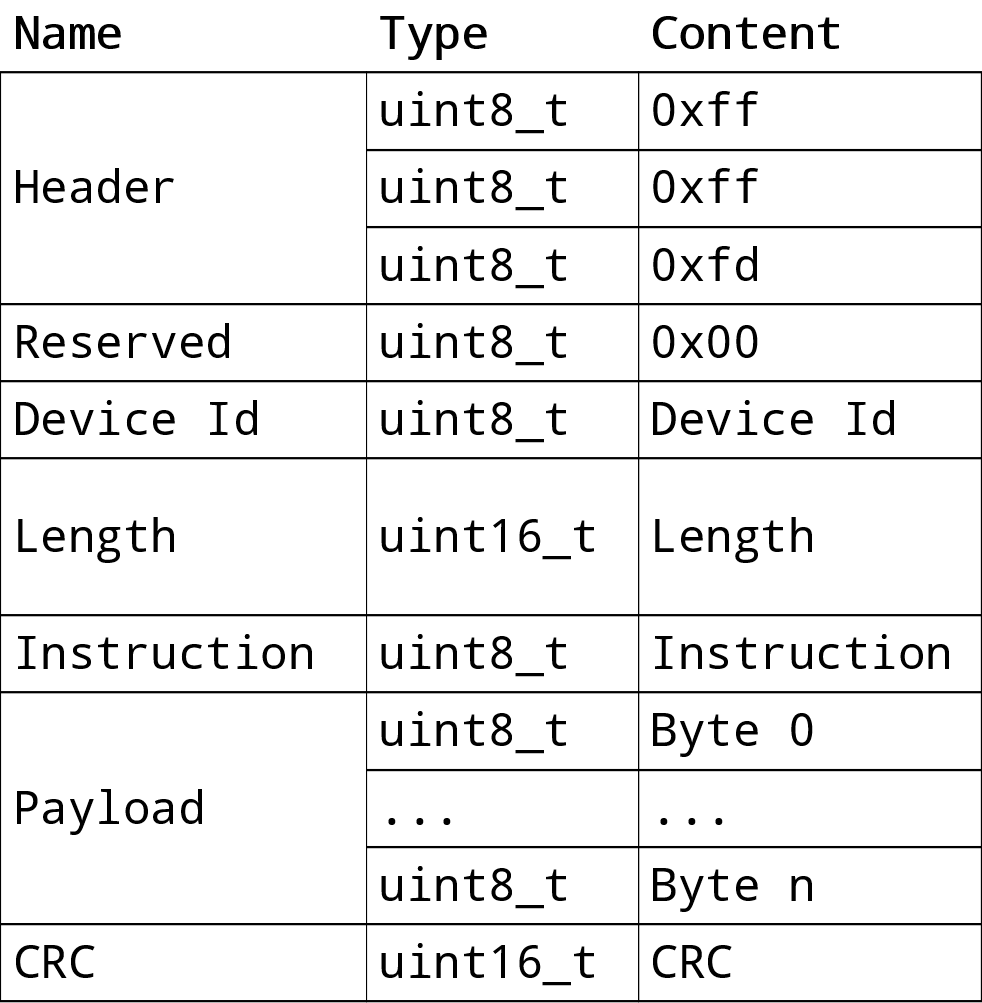
\includegraphics[scale=0.19]{img/packet.png}
        \caption{Generic layout of an instruction packet}
    \end{subfigure}%
    \begin{subfigure}[t]{0.5\textwidth}
        \centering
        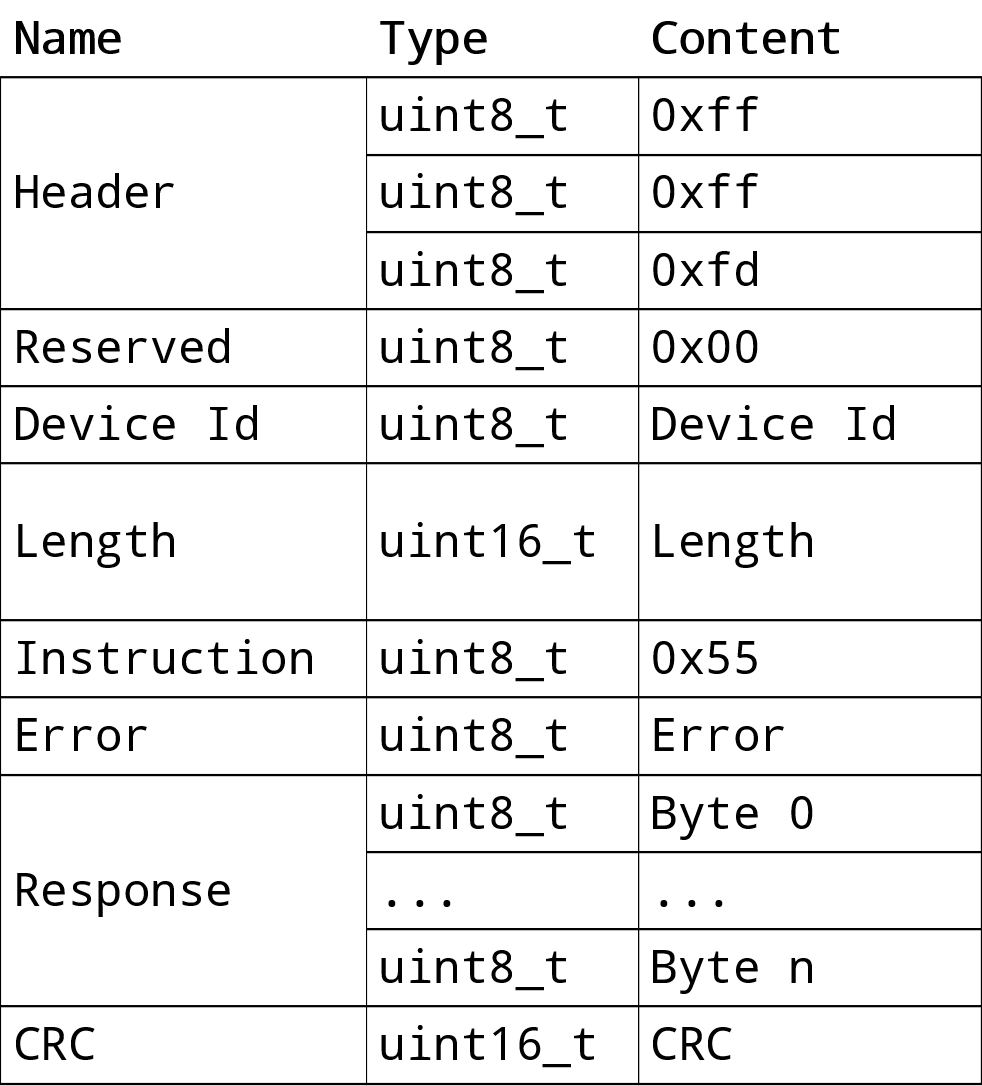
\includegraphics[scale=0.19]{img/status_packet.png}
        \caption{Generic layout of a status packet}
    \end{subfigure}

    \caption{Generic packet layout}
\end{figure}

Each packet has some metadata preceding the actual payload. It starts with a fixed byte sequence that allows
detecting a packet start without knowing where the last packet ended. It is followed by the device ID. For
instruction packets, this is the device that is targeted, for status packets it is the device that sent the
packet. The \textit{Length} field determines the remaining length of the packet. This allows for a payload of variable
size, depending on the instruction used or the data returned by the status packet. The next field is the instruction;
status packets use a reserved instruction. While the exact content of the payload varies, status packets always
store an additional error field as the first byte. This field can be used to indicate any errors that occurred
during the processing of an instruction.

Since the payload can contain arbitrary values, it can also contain the byte sequence used to mark the start of
a new packet. To prevent a receiver from misinterpreting this byte sequence, \textit{byte stuffing} is used.
Whenever a payload contains the byte sequence \lstinline{0xff 0xff 0xfd}, it is replaced by
\lstinline{0xff 0xff 0xfd 0xfd}. This makes it impossible to send a payload that could be interpreted as the
start of a new packet. The receiver simply removes the extra byte that was added. Note that the
\textit{Length} field specifies the number of bytes with byte stuffing already applied.

The last two bytes of every packet contain the \textit{CRC-16/BUYPASS}~\cite{crc-16-buypass} checksum of
every byte in the packet, including the starting sequence (and excluding the CRC itself). This checksum
can be used to detect transmission errors, in case the underlying bus does not have error detection
built-in (\textit{RS-485} does not).

\subsection{Instructions}
\label{basics/dynamixel-protocol/instructions}

\paragraph{Ping (\lstinline{0x01})}

Tests whether a device is connected. If the device ID is broadcast (\lstinline{0xfe}), all devices
respond. The status packet contains the device's model number and firmware version.

\begin{figure}[H]
    \centering
    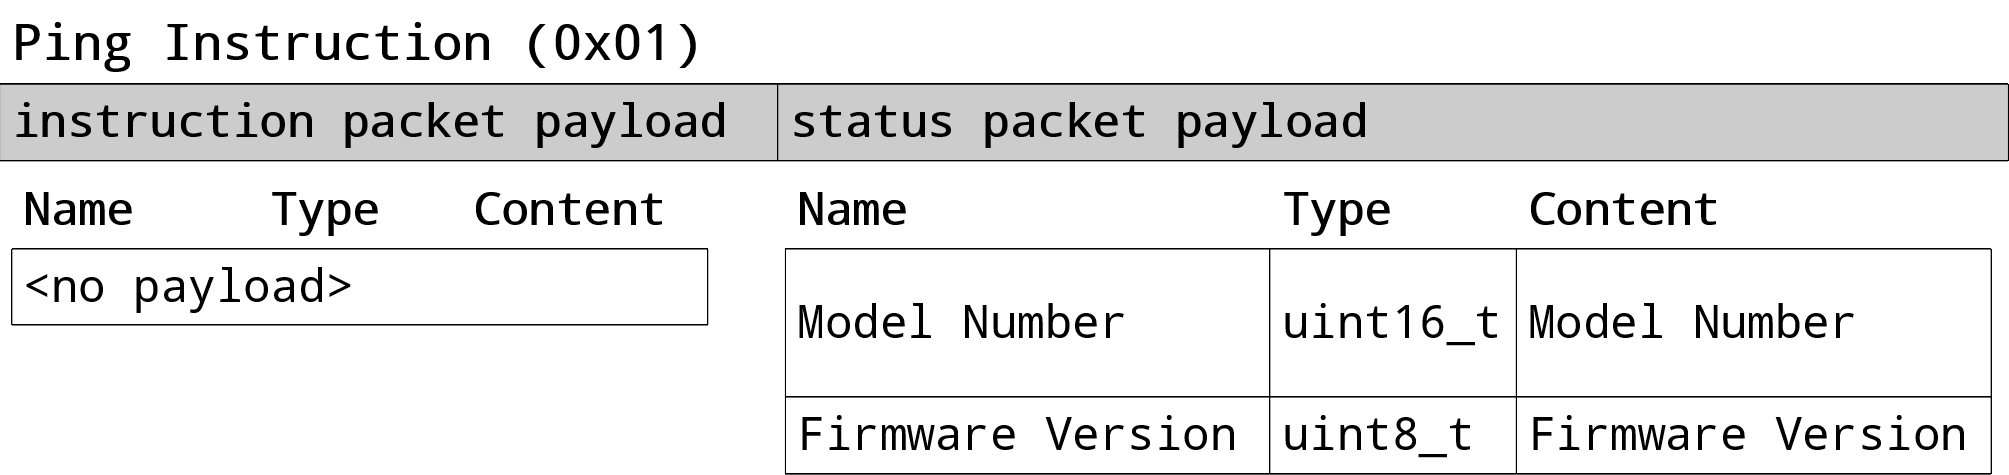
\includegraphics[scale=0.2]{img/ping_packet.png}
    \caption{\textit{Ping} instruction payloads}
\end{figure}

\paragraph{Read (\lstinline{0x02})}

Reads bytes from the \textit{control table} of a device. The status packet contains the requested
bytes.

\begin{figure}[H]
    \centering
    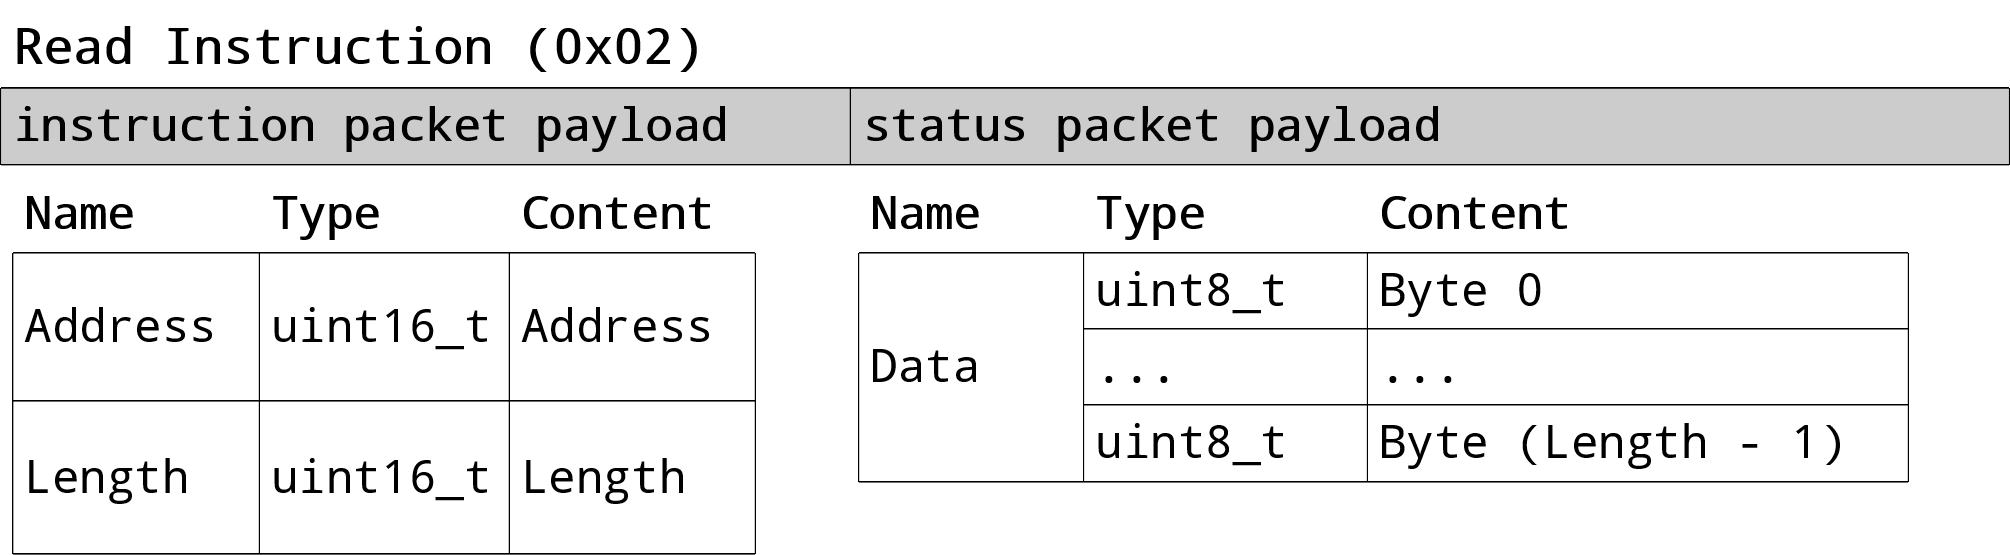
\includegraphics[scale=0.2]{img/read_packet.png}
    \caption{\textit{Read} instruction payloads}
\end{figure}

\paragraph{Write (\lstinline{0x03})}

Writes bytes to the \textit{control table} of a device. The status packet indicates whether the write
was executed successfully and contains no additional payload. Many devices can be configured to not
send any status packets on writes.

\begin{figure}[H]
    \centering
    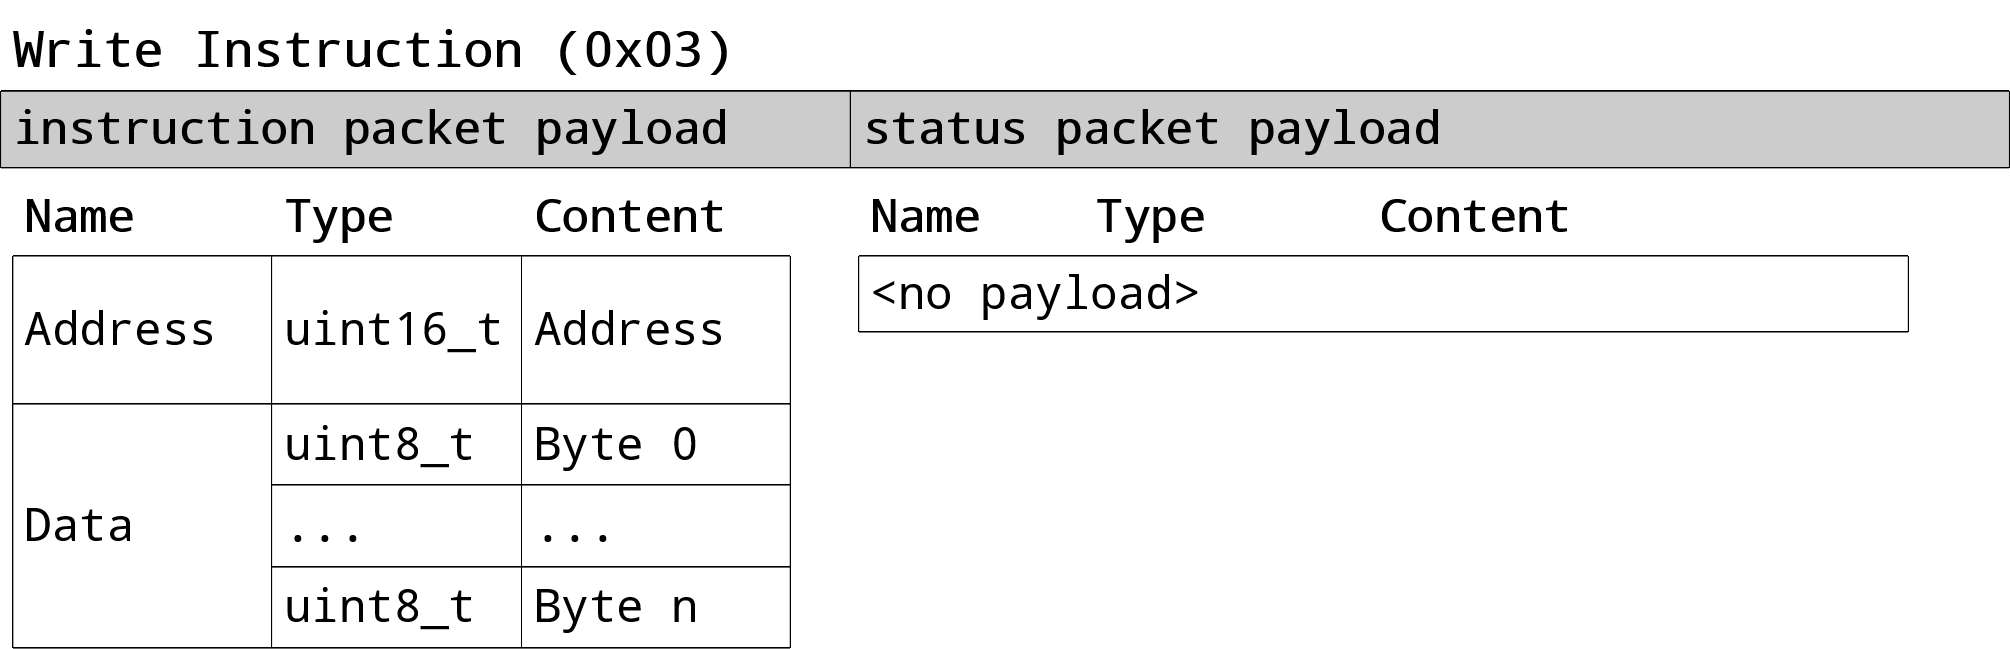
\includegraphics[scale=0.2]{img/write_packet.png}
    \caption{\textit{Write} instruction payloads}
\end{figure}

\paragraph{Reg Write (\lstinline{0x04})}

Identical to \textit{Write}, except that the write is delayed until an \textit{Action} instruction
is received.

\begin{figure}[H]
    \centering
    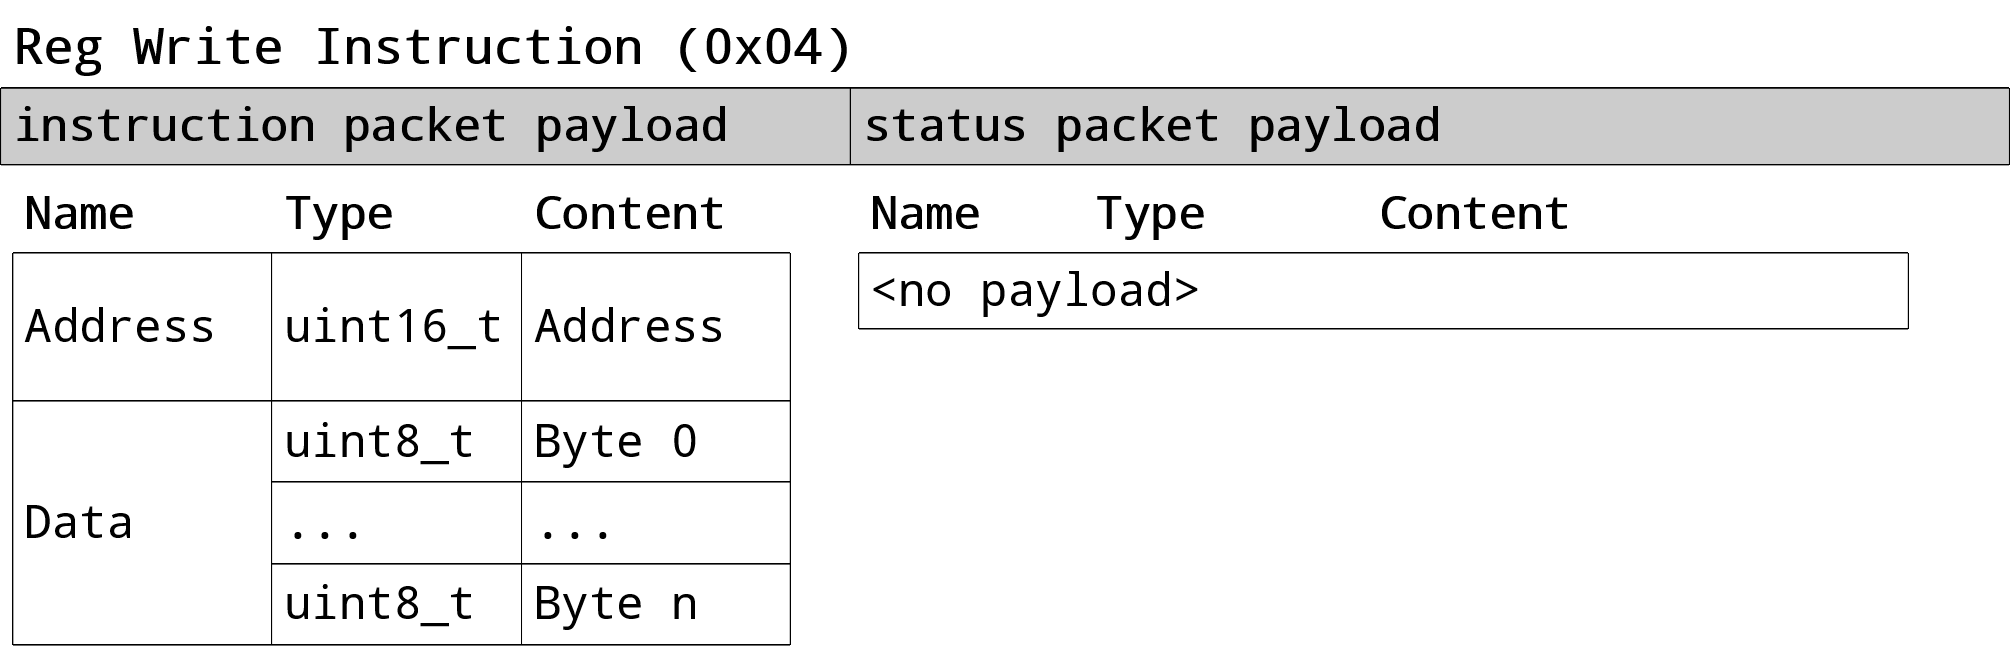
\includegraphics[scale=0.2]{img/reg_write_packet.png}
    \caption{\textit{Reg Write} instruction payloads}
\end{figure}

\paragraph{Action (\lstinline{0x05})}

Executes the write registered by the previous \textit{Reg Write} instruction. The status packet
indicates whether the write was executed successfully and contains no additional payload. Many
devices can be configured to not send any status packets on writes.

\begin{figure}[H]
    \centering
    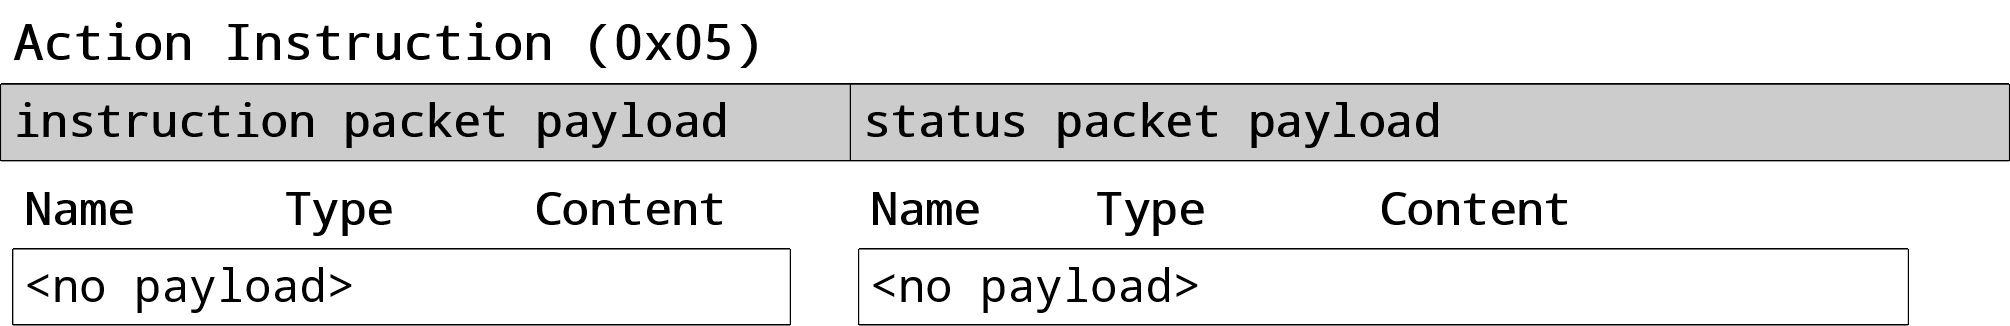
\includegraphics[scale=0.2]{img/action_packet.png}
    \caption{\textit{Action} instruction payloads}
\end{figure}

\paragraph{Factory Reset (\lstinline{0x06})}

Resets the device's \textit{control table} fields to their default values. \textit{Reset Mode}
determines the values that are reset:

\begin{itemize}
    \item \lstinline{0xff}: resets all values
    \item \lstinline{0x01}: resets all values except for the ID
    \item \lstinline{0x02}: resets all values except for the ID and the baud rate
\end{itemize}

The status packet indicates whether the reset was executed successfully and contains no additional
payload.

\begin{figure}[H]
    \centering
    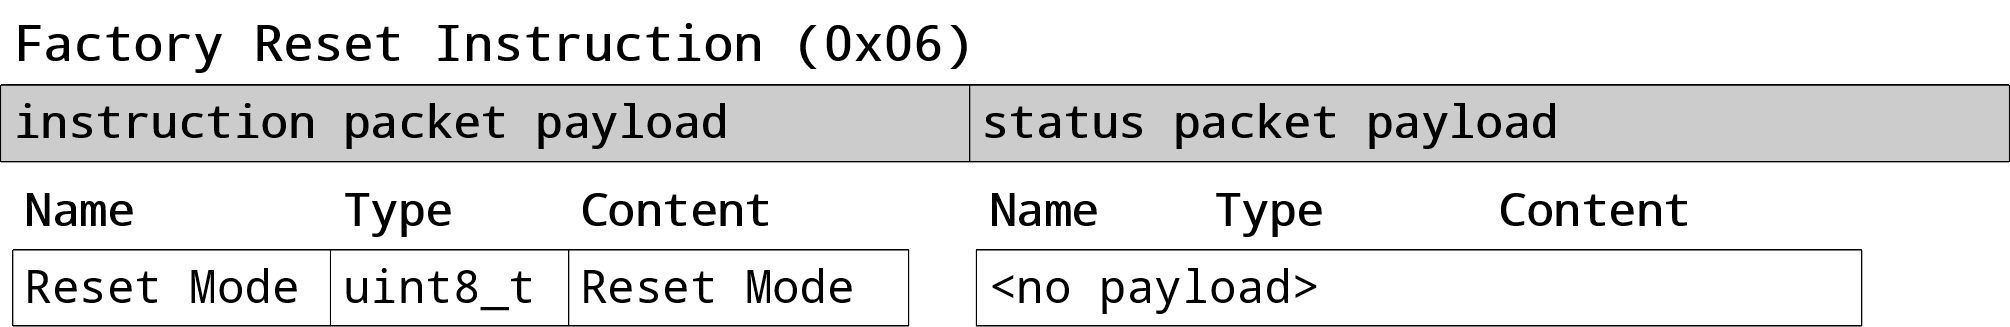
\includegraphics[scale=0.2]{img/factory_reset_packet.png}
    \caption{\textit{Factory Reset} instruction payloads}
\end{figure}

\paragraph{Reboot (\lstinline{0x08})}

Reboots the device. The status packet indicates whether the reboot was successful and contains no
additional payload.

\begin{figure}[H]
    \centering
    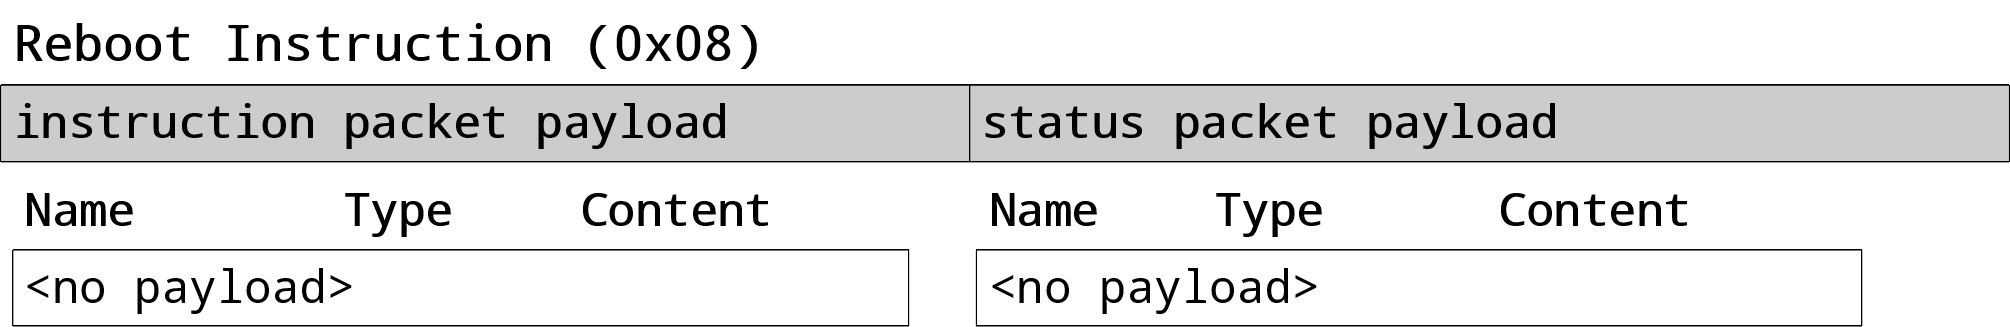
\includegraphics[scale=0.2]{img/reboot_packet.png}
    \caption{\textit{Reboot} instruction payloads}
\end{figure}

\paragraph{Clear (\lstinline{0x10})}

Resets the multi-turn information of the device. This instruction is very closely tied to servos
and generally not useful for other kinds of devices.

\begin{figure}[H]
    \centering
    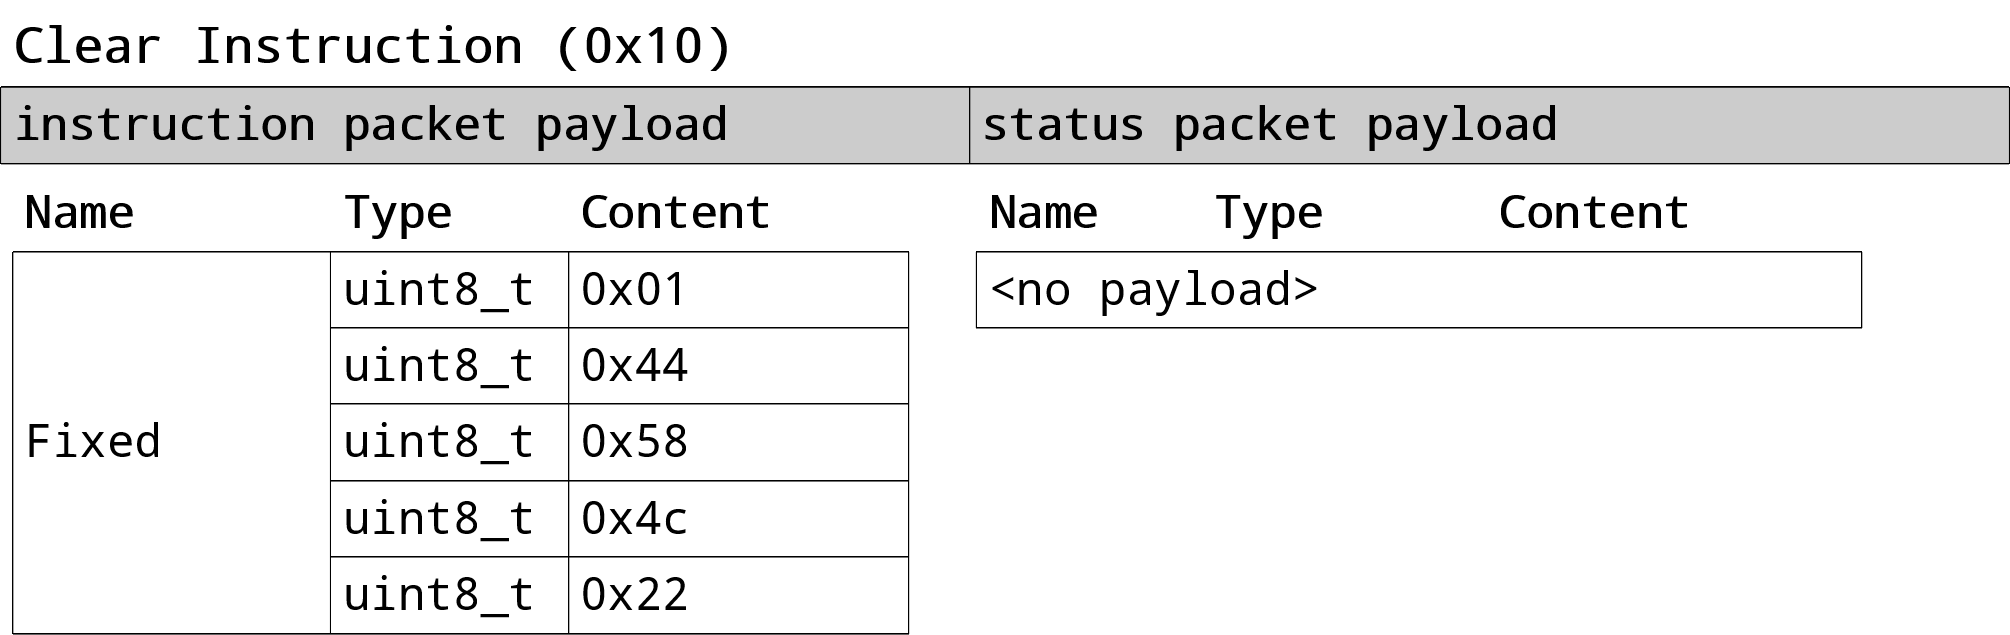
\includegraphics[scale=0.2]{img/clear_packet.png}
    \caption{\textit{Clear} instruction payloads}
\end{figure}

\paragraph{Sync Read (\lstinline{0x82})}

Reads bytes from the \textit{control tables} of multiple devices at once. The device ID of the
instruction packet must be broadcast (\lstinline{0xfe}). The status packet of each device contains
the requested bytes. Devices respond in the same order as their IDs in the instruction packet
payload.

\begin{figure}[H]
    \centering
    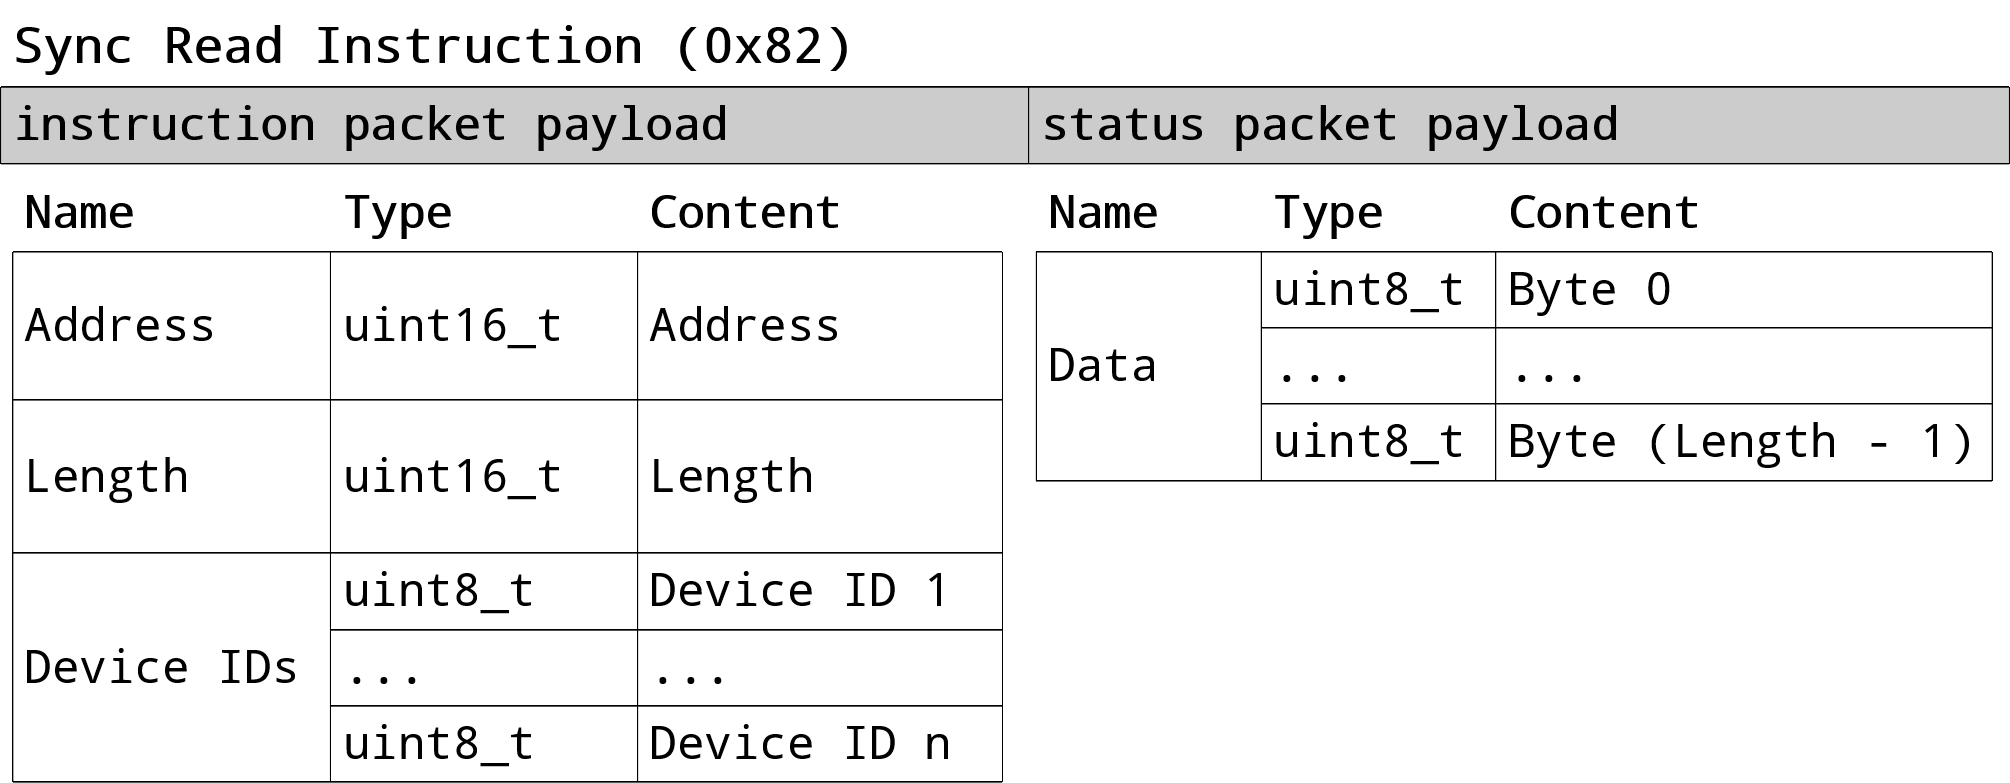
\includegraphics[scale=0.2]{img/sync_read_packet.png}
    \caption{\textit{Sync Read} instruction payloads}
\end{figure}

\clearpage
\paragraph{Sync Write (\lstinline{0x83})}

Writes bytes to the \textit{control tables} of multiple devices at once. The data for each device
can be different. The device ID of the instruction packet must be broadcast (\lstinline{0xfe}). The
status packet of each device indicates whether the write was executed successfully and contains no
additional payload. Devices respond in the same order as their IDs in the instruction packet
payload. Many devices can be configured to not send any status packets on writes.

\begin{figure}[H]
    \centering
    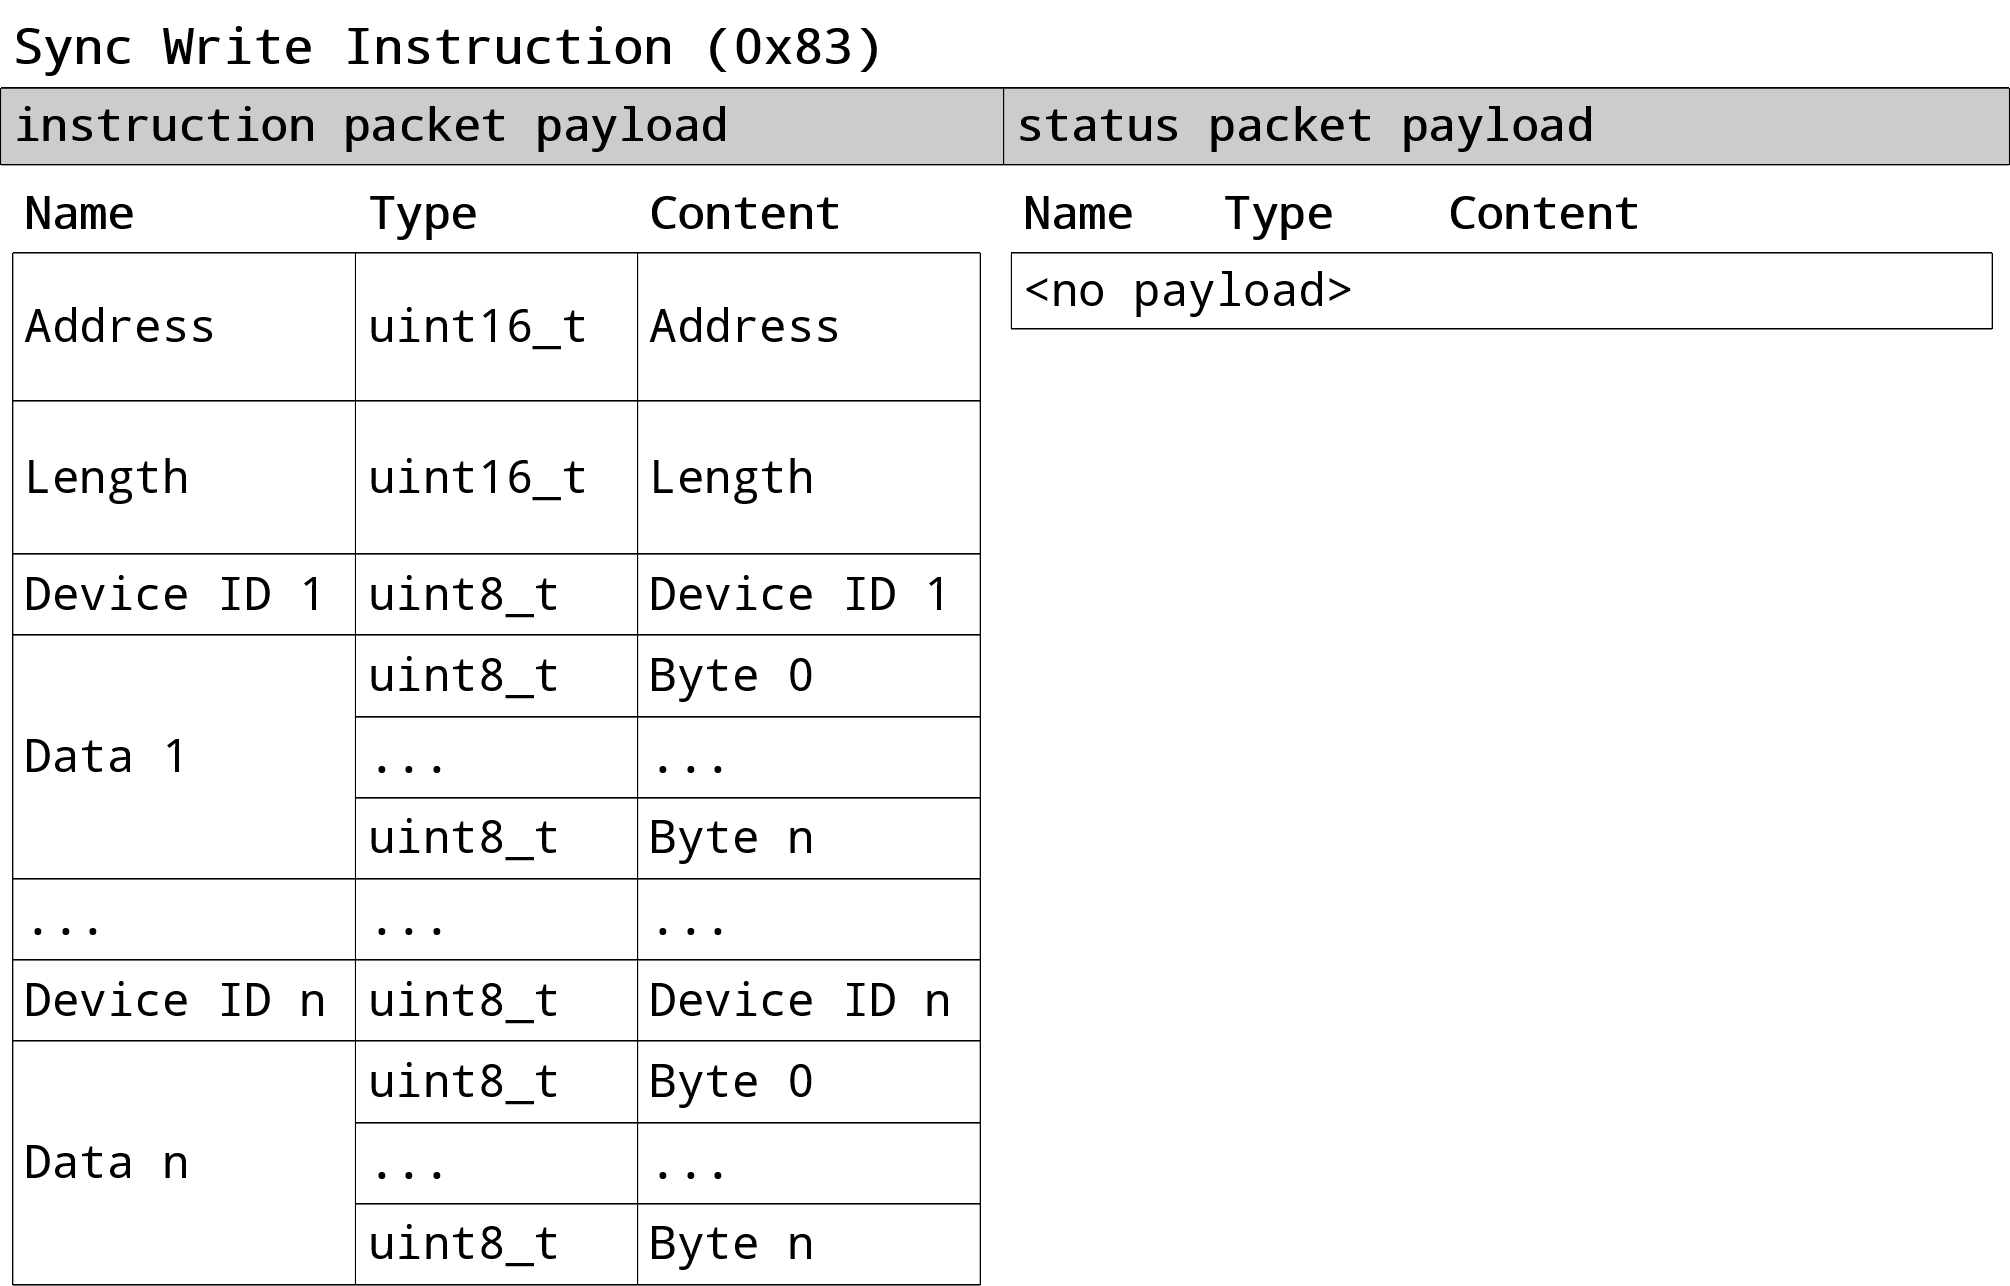
\includegraphics[scale=0.2]{img/sync_write_packet.png}
    \caption{\textit{Sync Write} instruction payloads}
\end{figure}

\clearpage
\paragraph{Bulk Read (\lstinline{0x92})}

Reads bytes from the \textit{control tables} of multiple devices at once. Unlike \textit{Sync Read},
this instruction allows for different addresses and lengths for each device. The device ID of the
instruction packet must be broadcast (\lstinline{0xfe}). The status packet of each device contains
the requested bytes. Devices respond in the same order as their IDs in the instruction packet
payload.

\begin{figure}[H]
    \centering
    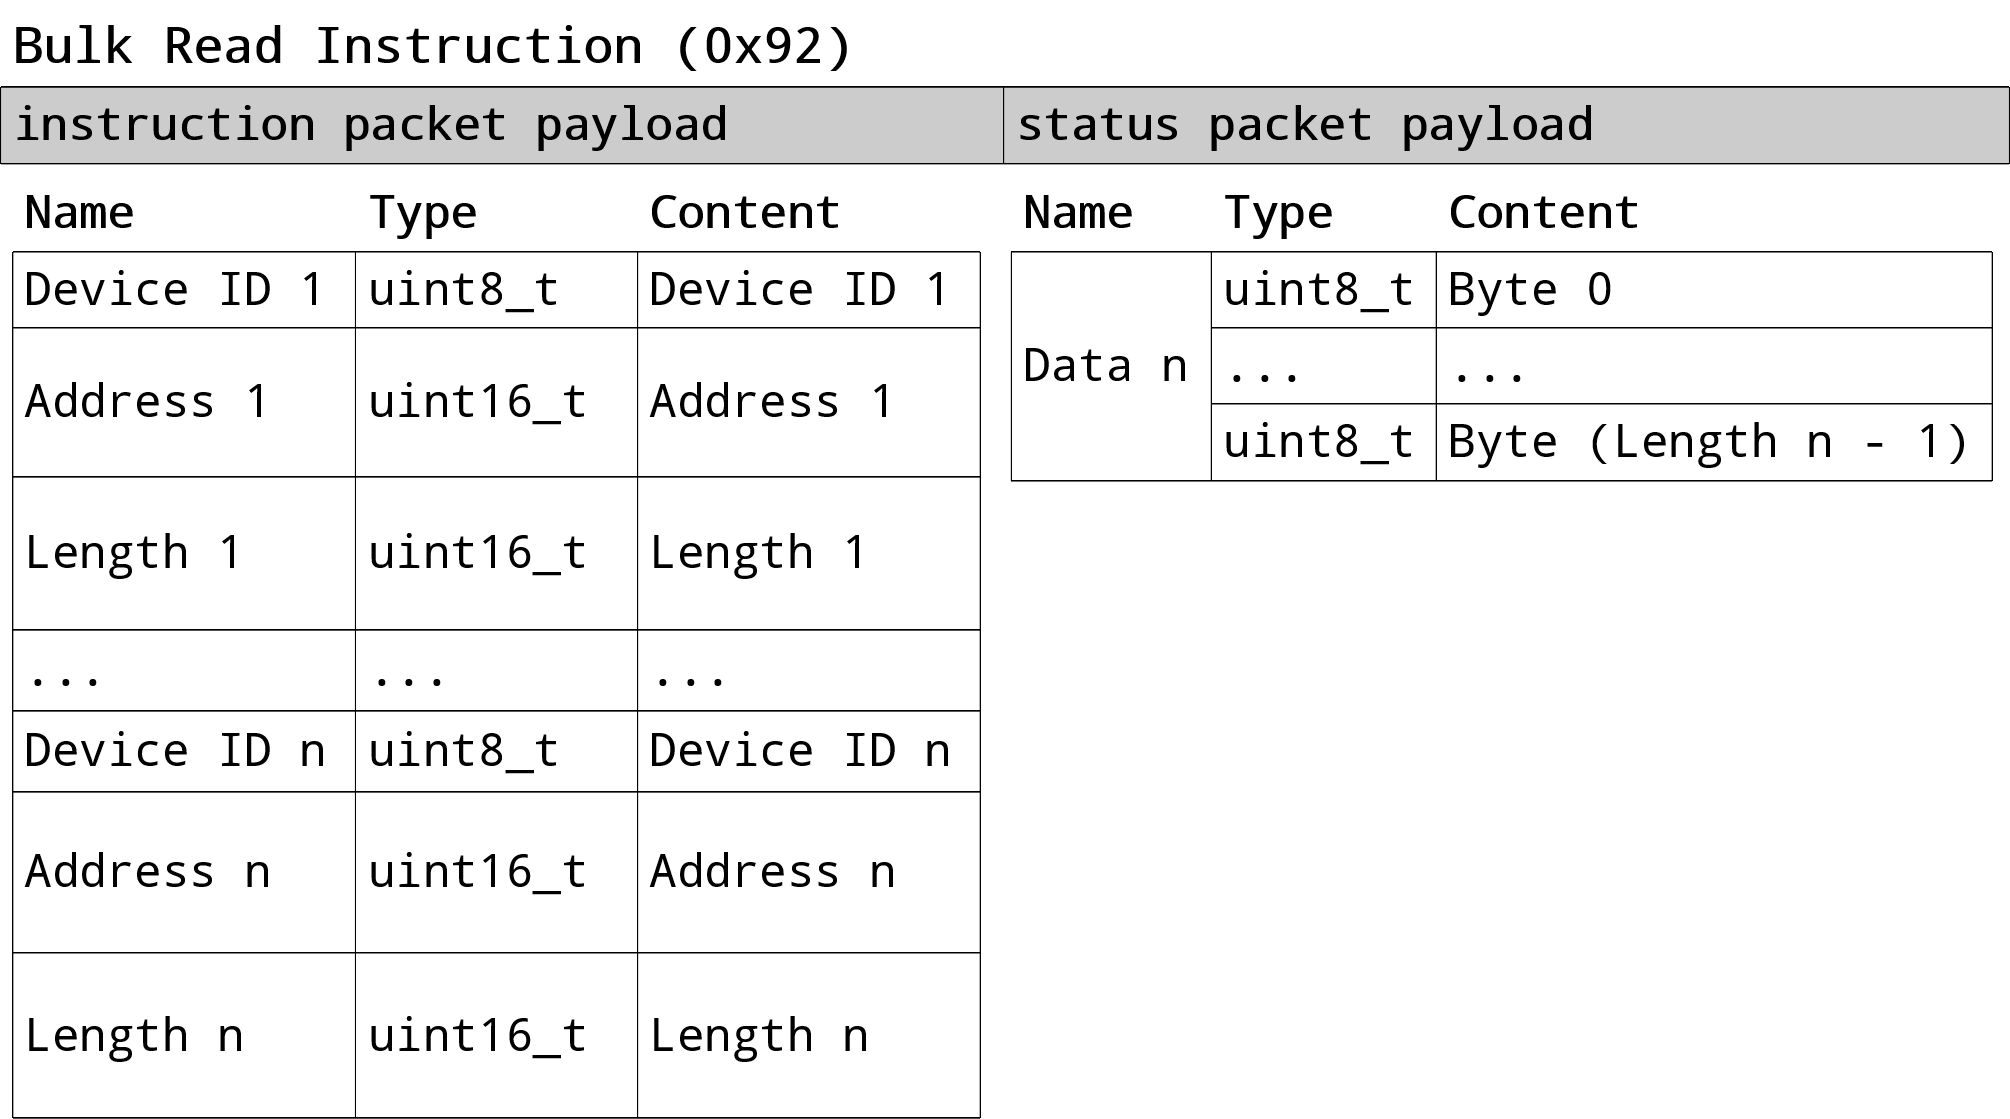
\includegraphics[scale=0.2]{img/bulk_read_packet.png}
    \caption{\textit{Bulk Read} instruction payloads}
\end{figure}

\clearpage
\paragraph{Bulk Write (\lstinline{0x93})}

Writes bytes to the \textit{control tables} of multiple devices at once. Unlike \textit{Sync Write},
this instruction allows not only for different data but also for different addresses and lengths for
each device. The device ID of the instruction packet must be broadcast (\lstinline{0xfe}). The status
packet of each device indicates whether the write was executed successfully and contains no additional
payload. Devices respond in the same order as their IDs in the instruction packet payload. Many
devices can be configured to not send any status packets on writes.

\begin{figure}[H]
    \centering
    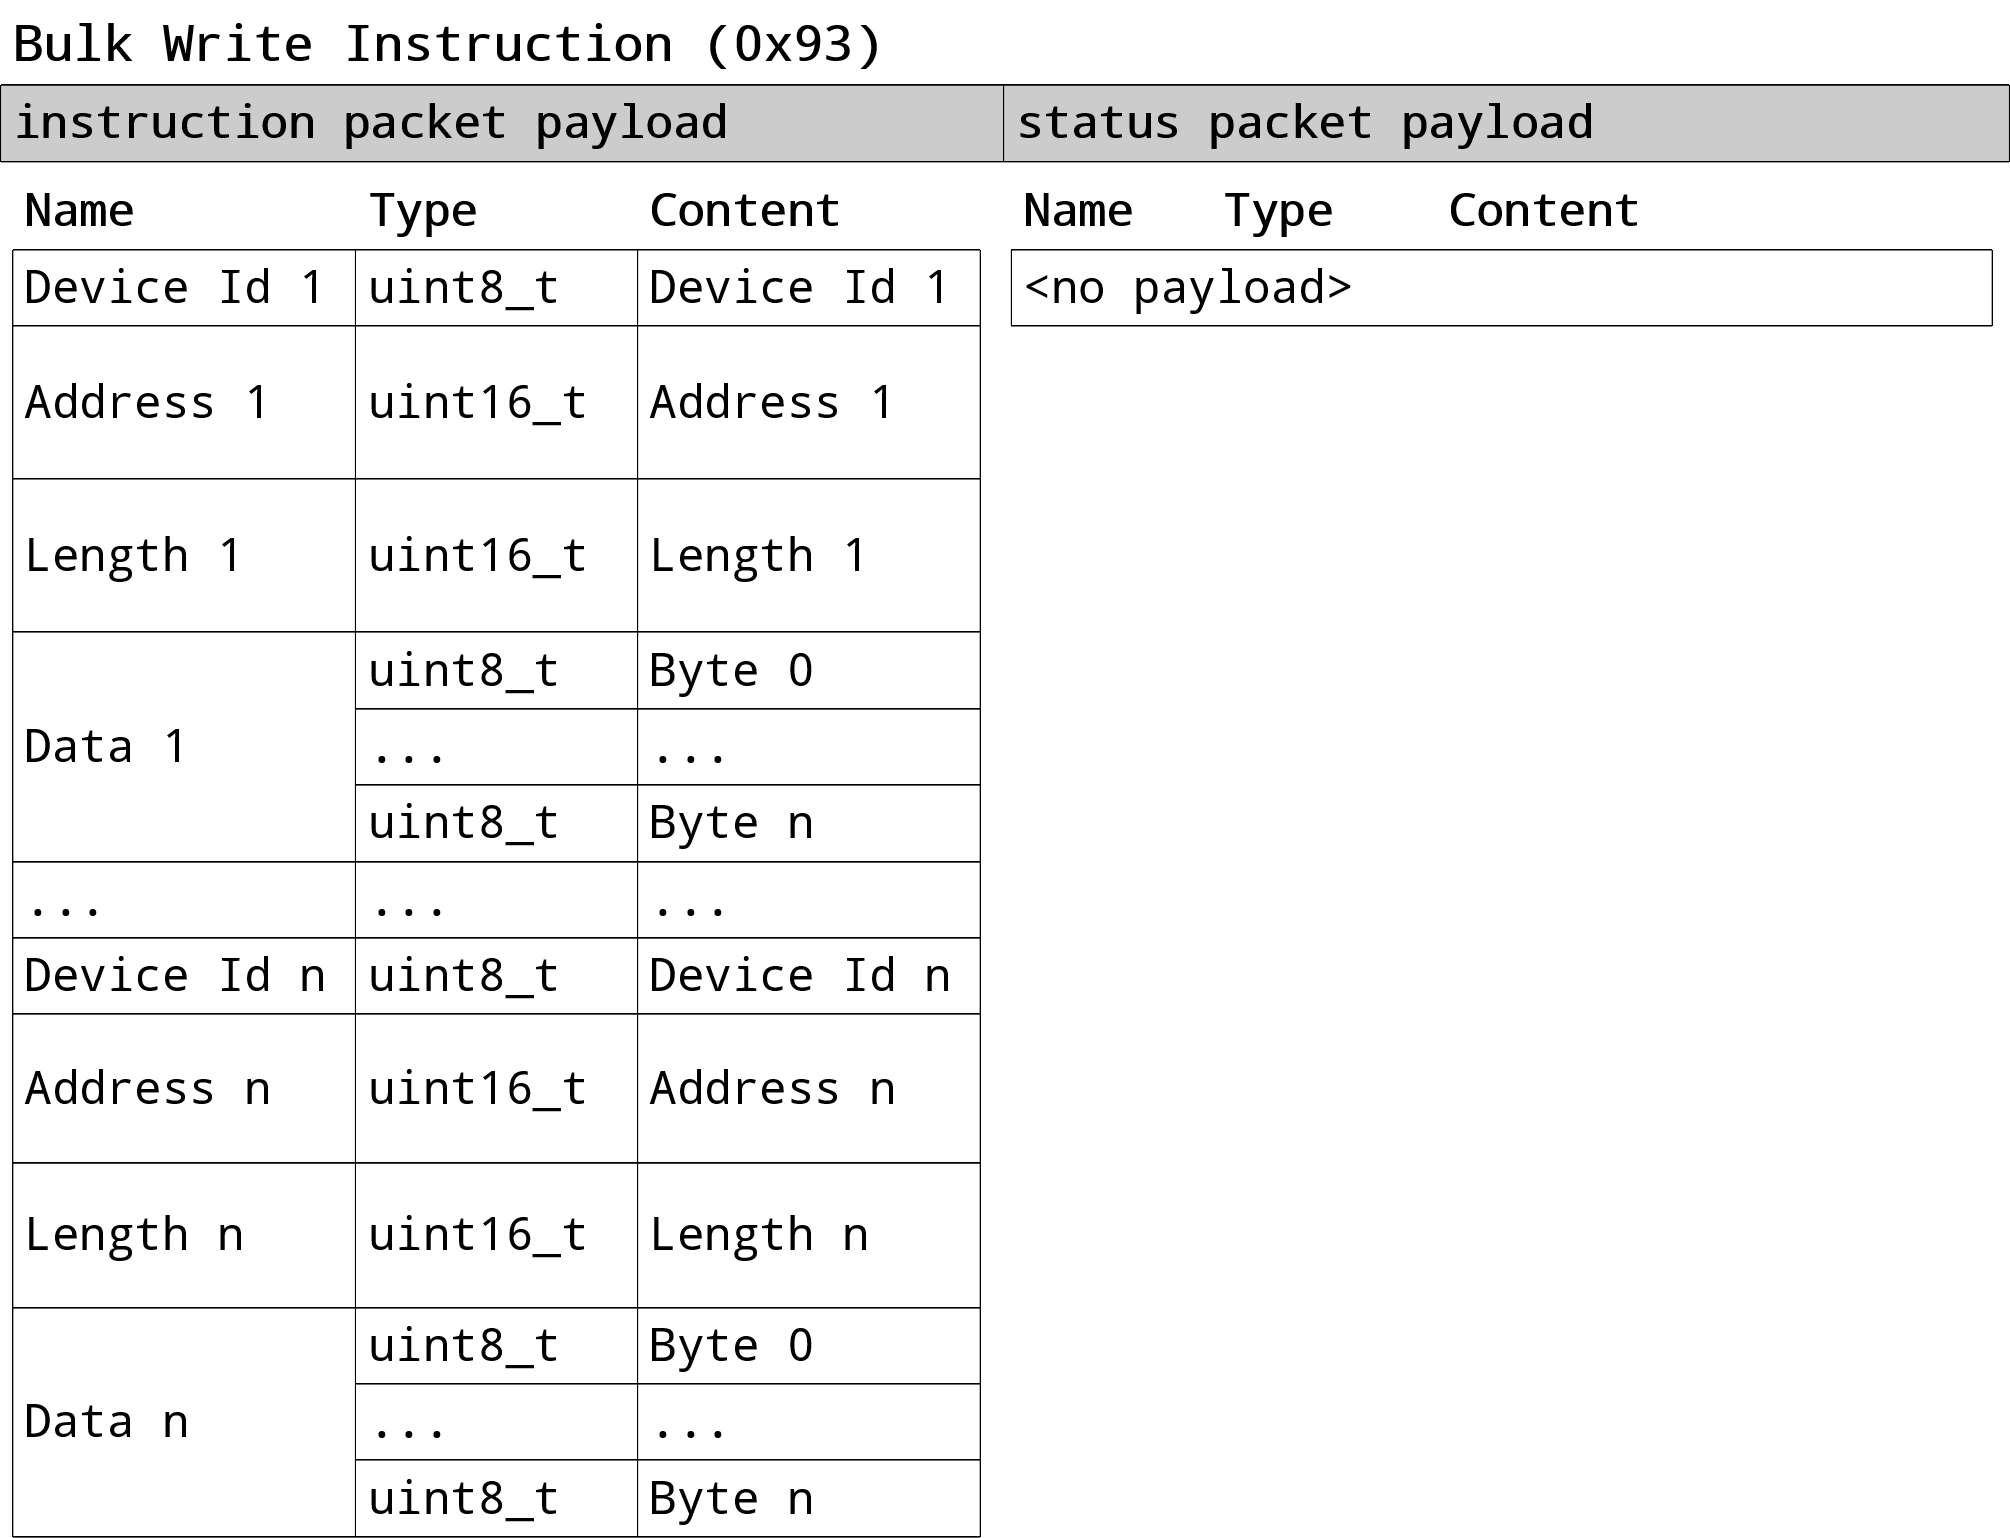
\includegraphics[scale=0.2]{img/bulk_write_packet.png}
    \caption{\textit{Bulk Write} instruction payloads}
\end{figure}

\subsection{Byte-Order}
\label{basics/dynamixel-protocol/byte-order}

All multi-byte values (packet fields, values in packet payloads and \textit{control table} fields) are
\textit{little-endian}. That is, for multi-byte values, the least significant byte comes first, then the
second least significant byte, etc.

\section{Embedded Operating Systems}
\label{basics/embedded-operating-systems}

Embedded operating systems are libraries linked directly with the user's code. They are small
both in runtime overhead and in program size, making them ideal for microcontrollers that cannot run
full operating systems like Linux or Windows. Embedded OSs only provide a small subset of the many
features offered by traditional operating systems. Common features are:

\begin{itemize}
    \item threads (sometimes also called tasks)
    \item concurrency primitives (mutexes, semaphores, queues, etc)
    \item memory allocators
    \item file systems
\end{itemize}

The most significant difference to traditional operating systems is the lack of security. Since the
operating system is part of the program itself, all code can be trusted and process boundaries are
not needed~\cite{modern-os-embedded-os}.

The core of an embedded OS are threads and context switching. Being part of the user program, the
application must configure an interrupt that calls the scheduler, which in turn runs application
code in one of the threads. Threads can run on separate CPU cores but they are also useful for single-core
systems. Threads are preemptive: one thread can be paused and another one started instead. This
makes it possible to guarantee that some threads always get the CPU time they need, for example to
process incoming data~\cite{freertos-fundamentals}.

The concurrent nature of threads makes it necessary to synchronize access to shared data. Since
synchronization is deeply intertwined with the scheduler, concurrency primitives must also be
provided by the embedded OS.
